\section{Machine Learning}~\label{sec.ML}

In this section, we will introduce the features we select and how we implement the machine learning.

Apparently, compared to the other features, the \textit{Tree Width} has much more impact on the run time. Thus we straightly group the data by tree width, and then for each group we do the polynomial linear regression.

Here is the features we may use:

\begin{enumerate}
    \item Average Bag Size: Average of size of bags on tree decomposition.
    \item Decomposition Overhead Ratio: Sum of bag size divided by size of graph.
    \item Average Depth: Average depth of tree.
    \item Node percentage: Introduce/Forget/Join/Leaf's Percentage of tree (sum of them is 100\%).
    \item Sum of Join node distance: Find all pairs of Join nodes and plus their distances.
    \item Branching Factor: Average number of childs (exclude leaf nodes).
    \item Bag Adjacency Factor: For all pair of nodes in a bag, that the adjacencent pairs divided by the total pairs.
    \item Bag Connectedness Factor: For all pair of nodes in a bag, the reachable pairs divided by the total pairs.
    \item Bag Neighborhood Coverage Factor: For all bags $B_{x}$, average of nodes that belong to a bag $B_{x}$ or are adjacencent to a node belongs to $B_{x}$
\end{enumerate}

After training, we use cross validation to validate each model and select the polynomial linear regression.

We select 2 best models to participate in the final test.

Model 1. For each tree width, we use Linear-Regression to predict the runtime.

\begin{figure}[h!]
    \centering
    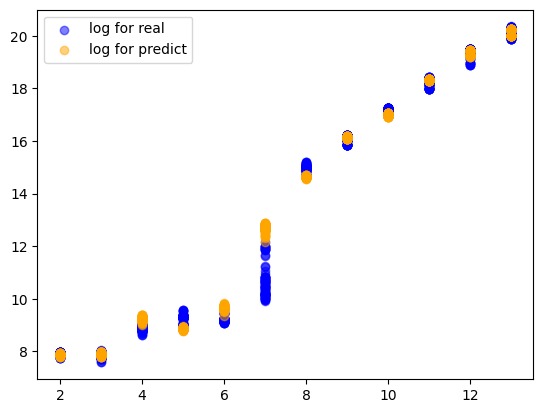
\includegraphics[width=0.24\textwidth]{model_polyLR.png}
    \caption{straight polynomial linear regression for run time}
    \label{straight polynomial linear regression for run time}
    \end{figure}

Model 2. For each tree width, we use Linear-Regression to predict the logarithmic runtime.

\begin{figure}[h!]
    \centering
    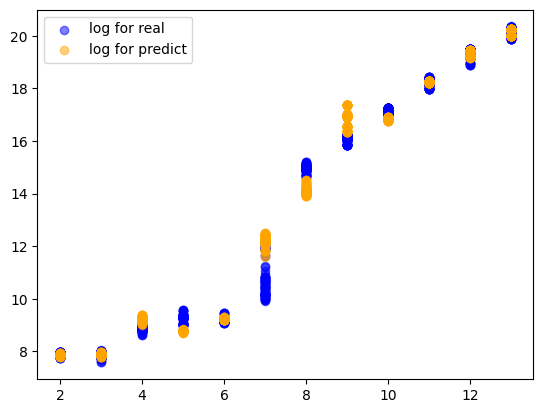
\includegraphics[width=0.24\textwidth]{model_lnpolyLR.png}
    \caption{polynomial linear regression for logarithmic runtime}
    \label{polynomial linear regression for logarithmic runtime}
    \end{figure}